\chapter{Berry Phase and Topological Band Theory}
\label{ch:topology}

The integer quantum Hall effect (Chapter~\ref{ch:qhe}) ended with a claim: the integer in $\sigma_H = \nu e^2/h$ is a topological invariant of the occupied states. This chapter builds the machinery behind that claim. An adiabatic change of a Hamiltonian produces a phase; that phase is a loop integral of a ``Berry vector potential'' on parameter space; its curl is a ``Berry magnetic field''; and degeneracies of the Hamiltonian act as magnetic monopoles. The integral of the Berry field over a closed surface is quantized (the Chern number), and is what the Hall conductance counts. The last sections work out the two-level problem and the massive Dirac Hamiltonian, ending with its anomalous Hall conductivity.

The structure is exactly that of the Aharonov--Bohm effect (Section 7.7 of the quantum mechanics notes): a vector potential defined up to a gauge, loop phases that are gauge invariant modulo $2\pi$, and a field that is exactly gauge invariant.

\begin{table}[ht]
\centering
\renewcommand{\arraystretch}{1.4}
\begin{tabular}{@{}lll@{}}
    \toprule
    & Electromagnetism (real space) & Berry phase (parameter space $\lvect{R}$)\\
    \midrule
    Potential & $\frac{q}{\hbar}\cvect{A}(\lvect{r})$ & $\bm{\mathcal{A}}_n(\lvect{R}) = i\langle n|\nabla_{\lvect{R}}n\rangle$\\
    Gauge freedom & $\psi\to e^{iq\Lambda/\hbar}\psi$ & $|n\rangle\to e^{i\delta(\lvect{R})}|n\rangle$\\
    Field & $\cvect{B} = \nabla\times\cvect{A}$ & $\bm{\Omega}_n = \nabla_{\lvect{R}}\times\bm{\mathcal{A}}_n$ (Berry curvature)\\
    Loop phase & $\frac q\hbar\oint\cvect{A}\cdot d\lvect{s}$ (mod $2\pi$) & $\gamma_n = \oint\bm{\mathcal{A}}_n\cdot d\lvect{R}$ (mod $2\pi$)\\
    Point source & magnetic monopole & degeneracy of $H(\lvect{R})$\\
    Quantized flux & Dirac: $4\pi e_M = N\Phi_0$ & Chern: $\oint\bm{\Omega}_n\cdot d\lvect{a} = 2\pi C_n$\\
    \bottomrule
\end{tabular}
\caption{The dictionary between electromagnetic potentials and Berry phase.}
\label{tab:berry-dictionary}
\end{table}

% ============================================================
\section{The Adiabatic Theorem and the Extra Phase}
% ============================================================

\subsection{Exact Equations for the Coefficients}

Let $H(t)$ have instantaneous, nondegenerate eigenstates,
\[
    H(t)|n;t\rangle = E_n(t)|n;t\rangle .
\]
At each moment these form a complete basis, so we may expand exactly, pulling out the phase each level would accumulate if $H$ were frozen (the \emph{dynamical phase}):
\[
    |\psi(t)\rangle = \sum_n c_n(t)\,e^{i\theta_n(t)}|n;t\rangle,
    \qquad
    \theta_n(t) = -\frac1\hbar\int_0^tE_n(t')\,dt',
    \qquad
    \dot\theta_n = -\frac{E_n}{\hbar}.
\]
Nothing here assumes $[H(t),H(t')] = 0$. If the Hamiltonians at different times did commute, they would share fixed eigenstates, every $\partial_t|n;t\rangle$ would vanish, and there would be no extra phase. The interesting case is precisely when the eigenstates rotate.

\paragraph{Step 1: substitute into $i\hbar\partial_t|\psi\rangle = H|\psi\rangle$.} The time derivative hits the coefficient, the phase and the ket. The phase term gives $i\hbar(i\dot\theta_n) = E_n$, which cancels $H|\psi\rangle$ term by term (that is why $\theta_n$ was pulled out), leaving
\[
    \sum_n e^{i\theta_n}\Bigl[\dot c_n|n;t\rangle + c_n|\partial_tn;t\rangle\Bigr] = 0 .
\]

\paragraph{Step 2: project onto $\langle m;t|$.}
\[
    \dot c_m = -c_m\langle m|\partial_tm\rangle - \sum_{n\neq m}c_n\,e^{i(\theta_n-\theta_m)}\langle m|\partial_tn\rangle .
\]

\paragraph{Step 3: rewrite the coupling.} Differentiate $H|n\rangle = E_n|n\rangle$ and project on $\langle m|$ with $m\neq n$:
\begin{equation}
    \langle m|\dot H|n\rangle + E_m\langle m|\partial_tn\rangle = E_n\langle m|\partial_tn\rangle
    \qquad\Longrightarrow\qquad
    \langle m|\partial_tn\rangle = \frac{\langle m|\dot H|n\rangle}{E_n-E_m}.
    \label{eq:berry-offdiag}
\end{equation}
This needs the levels to stay nondegenerate, which is the first hint that degeneracies are special.

\begin{formula}[Exact coefficient equation]
\[
    \dot c_m = -c_m\,\langle m|\partial_tm\rangle - \sum_{n\neq m}c_n\,e^{i(\theta_n-\theta_m)}\,\frac{\langle m|\dot H|n\rangle}{E_n-E_m}.
\]
\end{formula}

\subsection{The Adiabatic Approximation}

The second term transfers amplitude between levels. It is proportional to how fast $H$ changes, inversely proportional to the gap, and carries a phase oscillating at the gap frequency, so it averages away when
\[
    \frac{|\langle m|\dot H|n\rangle|}{|E_n-E_m|}\ll\frac{|E_n-E_m|}{\hbar}:
\]
the rate at which the eigenstates rotate must be small compared with the gap frequency. Dropping the term, a system that starts in level $n$ stays there.

\begin{theorem}[Adiabatic theorem]
\[
    \dot c_n = -c_n\langle n|\partial_tn\rangle
    \quad\Longrightarrow\quad
    |\psi(t)\rangle = e^{i\theta_n(t)}e^{i\gamma_n(t)}|n;t\rangle,
    \qquad
    \gamma_n(t) = i\int_0^t\langle n;t'|\partial_{t'}n;t'\rangle\,dt' .
\]
\end{theorem}

\paragraph{The extra phase is real.} Differentiating $\langle n|n\rangle = 1$ gives $\langle\partial_tn|n\rangle + \langle n|\partial_tn\rangle = 2\,\mathrm{Re}\langle n|\partial_tn\rangle = 0$. So $\langle n|\partial_tn\rangle$ is purely imaginary and $\gamma_n$ is real. It is a genuine phase, not a decay.

% ============================================================
\section{Berry Connection, Phase and Curvature}
% ============================================================

\subsection{From Time to Parameter Space}

Let $H$ depend on time only through a set of parameters, $H(t) = H(\lvect{R}(t))$. The chain rule gives
\[
    \frac{d}{dt}|n(\lvect{R}(t))\rangle = \bigl(\nabla_{\lvect{R}}|n\rangle\bigr)\cdot\dot{\lvect{R}},
\]
and $dt$ cancels from $\gamma_n$:

\begin{definition}[Berry connection and Berry phase]
\[
    \bm{\mathcal{A}}_n(\lvect{R}) = i\,\langle n(\lvect{R})|\nabla_{\lvect{R}}\,n(\lvect{R})\rangle,
    \qquad
    \gamma_n(C) = \int_C\bm{\mathcal{A}}_n\cdot d\lvect{R} .
\]
$\bm{\mathcal{A}}_n$ is real, by the argument above.
\end{definition}

\paragraph{Geometric versus dynamical.} Traverse the same path twice as fast: $\gamma_n$ is unchanged, because it depends only on the path in parameter space, while $\theta_n = -\frac1\hbar\int E_n\,dt$ halves. ``Geometric'' means independent of how fast the path is traversed, just like the Aharonov--Bohm phase.

In a crystal the natural parameter is the crystal momentum itself: $\lvect{R}\to\lvect{k}$ and $|n\rangle\to|u_{n\lvect{k}}\rangle$, the periodic part of the Bloch function, which is an eigenstate of the $\lvect{k}$-dependent Hamiltonian $H(\lvect{k}) = e^{-i\lvect{k}\cdot\lvect{r}}He^{i\lvect{k}\cdot\lvect{r}}$. A wavepacket driven through $\lvect{k}$-space by a force (Chapter~\ref{ch:semiclassical}) is precisely an adiabatic traversal of this parameter space.

\subsection{Gauge Freedom}

Eigenstates are defined only up to a phase, which may be chosen differently at each $\lvect{R}$:
\[
    |n(\lvect{R})\rangle\to e^{i\delta(\lvect{R})}|n(\lvect{R})\rangle
    \quad\Longrightarrow\quad
    \bm{\mathcal{A}}_n\to\bm{\mathcal{A}}_n - \nabla_{\lvect{R}}\delta,
    \qquad
    \gamma_n(C)\to\gamma_n(C) - \bigl[\delta(\text{end}) - \delta(\text{start})\bigr].
\]
\begin{itemize}
    \item \textbf{Open path:} $\gamma_n$ can be made anything, so it is not physical.
    \item \textbf{Closed loop:} the endpoint terms cancel, except that $\delta$ may wind by $2\pi N$ while $e^{i\delta}$ stays single-valued. Hence $\gamma_n(C)$ is gauge invariant modulo $2\pi$, exactly like the Aharonov--Bohm phase $\frac q\hbar\oint\cvect{A}\cdot d\lvect{s}$.
\end{itemize}

\subsection{Berry Curvature}

Stokes' theorem turns a loop phase into a flux, wherever the gauge is smooth on the enclosed surface:
\[
    \bm{\Omega}_n = \nabla_{\lvect{R}}\times\bm{\mathcal{A}}_n,
    \qquad
    \gamma_n(C) = \int_S\bm{\Omega}_n\cdot d\lvect{a} .
\]
The curvature is gauge invariant \emph{exactly}, not just modulo $2\pi$, since the curl of a gradient vanishes.

\paragraph{A derivative-free form.} Write $\bm{\Omega}_n = \nabla\times\bigl(i\langle n|\nabla n\rangle\bigr) = i\langle\nabla n|\times|\nabla n\rangle$ and insert a complete set of states. The $m = n$ term is $i\,\langle\nabla n|n\rangle\times\langle n|\nabla n\rangle$, the cross product of a purely imaginary vector with (minus) itself, which vanishes. For the others, \eqref{eq:berry-offdiag} with $\partial_t\to\nabla$ gives $\langle m|\nabla n\rangle = \langle m|\nabla H|n\rangle/(E_n-E_m)$:

\begin{theorem}[Gauge-invariant Berry curvature]
\[
    \bm{\Omega}_n = i\sum_{m\neq n}\frac{\langle n|\nabla_{\lvect{R}}H|m\rangle\times\langle m|\nabla_{\lvect{R}}H|n\rangle}{(E_n-E_m)^2}.
\]
\end{theorem}

No derivatives of states appear, so any phase convention gives the same answer. Two consequences:
\begin{enumerate}
    \item The curvature is large near near-degeneracies and singular at true degeneracies, which act as its sources.
    \item Swapping $n\leftrightarrow m$ flips the sign of each term (the cross product is antisymmetric), so $\sum_n\bm{\Omega}_n = 0$: the curvature of all bands together vanishes.
\end{enumerate}

% ============================================================
\section{The Two-Level Problem: Spin in a Field}
% ============================================================

\subsection{Setup and States}

Every two-band problem has the form $H = \lvect{d}\cdot\bm{\sigma}$ (plus a multiple of the identity, which does not affect eigenvectors), so this section covers all of them. Take first $H = -\lvect{d}\cdot\bm{\sigma}$, a spin in a field, with $\hat{\lvect{d}} = (\sin\theta\cos\phi,\sin\theta\sin\phi,\cos\theta)$. The ground state is aligned with $\hat{\lvect{d}}$:
\[
    |\chi\rangle = \cos\tfrac\theta2|{\uparrow}\rangle + \sin\tfrac\theta2\,e^{i\phi}|{\downarrow}\rangle .
\]

\paragraph{Where the gauge is singular.} Going around in $\phi$ is fine: $e^{i\phi}$ takes the same value at $0$ and $2\pi$. The trouble is at a pole, a single point where $\phi$ is undefined. At the south pole $|\chi\rangle = e^{i\phi}|{\downarrow}\rangle$: approaching along different meridians gives $|{\downarrow}\rangle$, $i|{\downarrow}\rangle$, $-|{\downarrow}\rangle$, \dots, so the ket has no single value there (like $(x+iy)/|x+iy|$ at the origin). The north pole is fine. The physical state at the south pole is fine; only the phase convention is singular.

\paragraph{Fixing it.} Multiply by a phase that is single-valued on every circle of constant $\theta$, i.e.\ one that winds by an integer multiple of $2\pi$. The choice $e^{-i\phi}$ gives
\[
    |\chi'\rangle = e^{-i\phi}|\chi\rangle = \cos\tfrac\theta2\,e^{-i\phi}|{\uparrow}\rangle + \sin\tfrac\theta2|{\downarrow}\rangle,
\]
smooth at the south pole but now singular at the north pole. The singularity moved; it did not disappear. Section~\ref{sec:no-smooth-gauge} proves it cannot.

\begin{fact}[A tempting fix that fails]
A phase with fractional winding such as $e^{-i\theta\phi/\pi}$ cures both poles, but it is no longer single-valued in $\phi$ for $0<\theta<\pi$: $e^{-2i\theta}\neq1$. It trades a bad point for a bad meridian.
\end{fact}

\subsection{Connection, Phase and Curvature}

Use coordinate components, $\gamma = \oint(\mathcal{A}_\theta\,d\theta + \mathcal{A}_\phi\,d\phi)$ with $\mathcal{A}_\mu = i\langle\chi|\partial_\mu\chi\rangle$. For $|\chi\rangle$ the $\theta$ dependence is only in real amplitudes, so $\mathcal{A}_\theta = \cos\frac\theta2\,\partial_\theta\cos\frac\theta2 + \sin\frac\theta2\,\partial_\theta\sin\frac\theta2$ times $i$, which is $\frac i2\partial_\theta(1) = 0$. Only the lower component depends on $\phi$:
\[
    \mathcal{A}_\theta = 0,
    \qquad
    \mathcal{A}_\phi = i\bigl(i\sin^2\tfrac\theta2\bigr) = -\sin^2\tfrac\theta2 = -\frac{1-\cos\theta}{2}.
\]
If a connection comes out imaginary, an overall factor of $i$ was dropped.

\paragraph{Loops.} Along meridians only $\mathcal{A}_\theta = 0$ contributes, so for any loop made of meridians and an arc of latitude only the latitude arc counts. On the equator $\mathcal{A}_\phi = -\frac12$:
\[
    \gamma_{\text{hemisphere}} = \int_0^{2\pi}\mathcal{A}_\phi\big|_{\pi/2}\,d\phi = -\pi,
    \qquad
    \gamma_{\text{octant}} = \int_0^{\pi/2}\mathcal{A}_\phi\big|_{\pi/2}\,d\phi = -\frac\pi4 .
\]
The octant loop runs from the north pole down a meridian, a quarter of the way around the equator, and back up. The hemisphere alone cannot fix the sign ($-\pi\equiv\pi$); the octant can.

\paragraph{Curvature per solid angle.} In coordinate components $F = \partial_\theta\mathcal{A}_\phi - \partial_\phi\mathcal{A}_\theta = -\frac12\sin\theta$. The Berry phase of a small coordinate rectangle is $F\,d\theta\,d\phi$, while its solid angle is $d\Omega = \sin\theta\,d\theta\,d\phi$, so the curvature per unit solid angle is a constant.

\begin{formula}[Spin one-half: half the solid angle]
\[
    \frac{F}{\sin\theta} = -\frac12,
    \qquad
    \gamma(C) = -\tfrac12\,\Omega(C)\quad(\text{state aligned with }\hat{\lvect{d}}).
\]
For the state anti-aligned with $\hat{\lvect{d}}$ the sign flips: $+\frac12$ per solid angle.
\end{formula}

Check: $-\frac12\cdot2\pi = -\pi$ (hemisphere) and $-\frac12\cdot\frac{4\pi}{8} = -\frac\pi4$ (octant).

\begin{figure}[ht]
\centering
\begin{tikzpicture}[>=Stealth,scale=1.6]
  \shade[ball color=blue!8] (0,0) circle (1);
  \draw (0,0) circle (1);
  \draw[gray] (-1,0) arc (180:360:1 and 0.3);
  \draw[gray,dashed] (1,0) arc (0:180:1 and 0.3);
  % octant loop: north pole -> (1,0) direction -> front point -> north pole
  \fill[red!25,opacity=0.6] (0,1) -- (0,1) arc (90:0:0.55 and 1) -- (0.55,-0.25) arc (-63:-90:1 and 0.3) .. controls (0.0,0.3) .. (0,1);
  \draw[thick,red!70!black,->] (0,1) arc (90:0:0.55 and 1);
  \draw[thick,red!70!black,->] (0.55,0) .. controls (0.45,-0.18) .. (0,-0.3);
  \draw[thick,red!70!black,->] (0,-0.3) .. controls (0.03,0.4) .. (0,1);
  \fill (0,1) circle (0.025) node[above]{N};
  \draw[->,thick] (0,0) -- (0.5,0.55) node[right]{$\hat{\lvect{d}}$};
  \node[red!70!black] at (1.45,0.65) {$\gamma = -\tfrac12\Omega$};
\end{tikzpicture}
\caption{The Berry phase of a spin-$\frac12$ state aligned with $\hat{\lvect{d}}$, for a loop traced by $\hat{\lvect{d}}$ on the unit sphere, is $-\frac12$ times the solid angle enclosed. The loop shown encloses one octant, $\Omega = \pi/2$.}
\label{fig:berry-octant}
\end{figure}

\begin{fact}[Coordinate versus physical components]
$\mathcal{A}_\phi = i\langle\chi|\partial_\phi\chi\rangle$ is the coefficient of $d\phi$. The textbook spherical curl uses physical components along unit vectors, related on the unit sphere by $\mathcal{A}_\phi^{\text{phys}} = \mathcal{A}_\phi/\sin\theta$. Feeding coordinate components into the physical-component curl inserts a spurious $\sin\theta$. Either use $F = \partial_\theta\mathcal{A}_\phi - \partial_\phi\mathcal{A}_\theta$ directly, or convert first.
\end{fact}

\subsection{Two Gauges, Same Physics}

For $|\chi'\rangle = e^{-i\phi}|\chi\rangle$ the extra factor contributes $i\cdot(-i) = 1$ to $\mathcal{A}_\phi$, so $\mathcal{A}'_\phi = 1 - \sin^2\frac\theta2 = \cos^2\frac\theta2$, $\mathcal{A}'_\theta = 0$, and again $F/\sin\theta = -\frac12$. The difference is a pure gradient,
\[
    \mathcal{A}'_\phi - \mathcal{A}_\phi = \cos^2\tfrac\theta2 + \sin^2\tfrac\theta2 = 1 = \partial_\phi\phi,
    \qquad
    \oint(\bm{\mathcal{A}}' - \bm{\mathcal{A}})\cdot d\lvect{R} = \oint d\phi = 2\pi n,
\]
with $n$ the winding of the loop around the $z$-axis. Closed-loop phases agree modulo $2\pi$ (equator: $-\pi$ versus $+\pi$); curvatures agree exactly.

% ============================================================
\section{Monopoles and the Obstruction to a Smooth Gauge}
% ============================================================

\subsection{Dirac's Magnetic Monopole}

In Gaussian units, a monopole has $\cvect{B} = e_M\rhat/r^2$ and total flux $4\pi e_M$ through any sphere around it.

\paragraph{No single smooth $\cvect{A}$.} Suppose one $\cvect{A}$ were smooth on the whole sphere. Cut along the equator. With outward normals, the boundaries of the two caps run around the equator in opposite directions, so Stokes' theorem gives
\[
    \Phi_N + \Phi_S = \oint_{\text{eq}}\cvect{A}\cdot d\lvect{s} - \oint_{\text{eq}}\cvect{A}\cdot d\lvect{s} = 0\neq4\pi e_M .
\]

\paragraph{Two patches.} Each of the following potentials is singular on one half of the $z$-axis (the Dirac string):
\[
    \cvect{A}^{(\mathrm{I})} = \frac{e_M(1-\cos\theta)}{r\sin\theta}\hat{\bm{\phi}}\quad(\text{bad at }\theta = \pi),
    \qquad
    \cvect{A}^{(\mathrm{II})} = -\frac{e_M(1+\cos\theta)}{r\sin\theta}\hat{\bm{\phi}}\quad(\text{bad at }\theta = 0).
\]
On the overlap $\cvect{A}^{(\mathrm{II})} - \cvect{A}^{(\mathrm{I})} = -\frac{2e_M}{r\sin\theta}\hat{\bm{\phi}} = \nabla\Lambda$ with $\Lambda = -2e_M\phi$. A particle of charge $e$ has wavefunctions in the two gauges that differ by $e^{ie\Lambda/\hbar c} = e^{-2iee_M\phi/\hbar c}$, and single-valuedness around the equator demands:

\begin{theorem}[Dirac quantization]
\[
    \frac{2ee_M}{\hbar c} = N\in\mathbb{Z}
    \qquad\Longleftrightarrow\qquad
    4\pi e_M = N\Phi_0,
    \qquad
    \Phi_0 = \frac{2\pi\hbar c}{e}.
\]
The total flux is a whole number of flux quanta, and the Dirac string's Aharonov--Bohm phase $2\pi N$ is invisible.
\end{theorem}

\subsection{The Spin-\texorpdfstring{$\tfrac12$}{1/2} Berry Phase Is a Monopole}

In physical components on the unit sphere, the two spin gauges give $\mathcal{A}^{\text{phys}}_\phi = -\frac{1-\cos\theta}{2\sin\theta}$ and $+\frac{1+\cos\theta}{2\sin\theta}$: exactly the two patches above with $e_M = -\frac12$ and $r = 1$. The degeneracy at $\lvect{d} = 0$, where the two levels meet, is the monopole.

\begin{table}[ht]
\centering
\renewcommand{\arraystretch}{1.3}
\begin{tabular}{@{}lll@{}}
    \toprule
    & Magnetic monopole & Spin-$\frac12$ Berry phase\\
    \midrule
    Source & magnetic charge at origin & degeneracy at $\lvect{d} = 0$\\
    Strength & $e_M$ & $-\frac12$ (aligned state)\\
    Patch singular at south pole & $\cvect{A}^{(\mathrm{I})}$ & $|\chi\rangle$\\
    Patch singular at north pole & $\cvect{A}^{(\mathrm{II})}$ & $|\chi'\rangle = e^{-i\phi}|\chi\rangle$\\
    Gluing function & $\Lambda = -2e_M\phi$ & $\delta = -\phi$\\
    Total flux & $4\pi e_M$ & $-\frac12\cdot4\pi = -2\pi$\\
    Quantization & $N\Phi_0$ & $2\pi C$, here $C = -1$\\
    \bottomrule
\end{tabular}
\caption{The spin-$\frac12$ Berry connection is a Dirac monopole in parameter space.}
\end{table}

\subsection{No Globally Smooth Gauge}
\label{sec:no-smooth-gauge}

Suppose some gauge were smooth on the whole sphere. Then with that single connection the equator is traversed in opposite senses as the boundary of the two caps,
\[
    \gamma_N = \int_{\phi=0}^{2\pi}\mathcal{A}_\phi\big|_{\pi/2}\,d\phi,
    \qquad
    \gamma_S = \int_{\phi=2\pi}^{0}\mathcal{A}_\phi\big|_{\pi/2}\,d\phi = -\gamma_N,
\]
so by Stokes the total curvature would be $\gamma_N + \gamma_S = 0$. But the curvature is gauge invariant, and in any gauge
\[
    \int_{S^2}\frac{F}{\sin\theta}\,d\Omega = -\tfrac12\cdot4\pi = -2\pi\neq0 .
\]
This is a contradiction, so no smooth global gauge exists.

\begin{fact}[State the contradiction with the curvature integral, not with phases]
Phases live modulo $2\pi$, and $-2\pi\equiv0$, so ``the phases should add to $-2\pi$ but add to $0$'' is not a contradiction. The integral of the curvature is a real number with no $2\pi$ ambiguity; that is the quantity a smooth gauge forces to be $0$ and that is actually $-2\pi$. Also note that $\gamma_S = -\gamma_N$ is a statement about the \emph{line} integrals of one smooth connection. The \emph{surface} integrals of the curvature over the two caps are both $-\pi$, not opposite.
\end{fact}

\begin{theorem}[Chern number]
For any closed surface $S$ in parameter space on which band $n$ stays nondegenerate,
\[
    \oint_S\bm{\Omega}_n\cdot d\lvect{a} = 2\pi C_n,
    \qquad
    C_n\in\mathbb{Z}\quad(\text{the first Chern number}).
\]
A smooth global gauge forces $C_n = 0$. A nonzero Chern number is the obstruction, just as a nonzero magnetic charge rules out a single smooth vector potential.
\end{theorem}

\paragraph{Why an integer.} Cover $S$ with two patches, each with a smooth gauge, glued along a loop by $e^{i\delta}$. The flux through the two patches is the difference of their loop phases, $\oint\nabla\delta\cdot d\lvect{R}$, and single-valuedness of $e^{i\delta}$ makes this $2\pi$ times an integer: the winding of the gluing phase.

\paragraph{The two-dimensional Brillouin zone.} The Brillouin zone of a 2D crystal is a torus: $\lvect{k}$ and $\lvect{k}+\cvect{G}$ label the same state. It is a closed surface, so each isolated band has an integer Chern number $C_n = \frac{1}{2\pi}\int_{\text{BZ}}\Omega_n\,d^2k$. This is the TKNN integer of the quantum Hall effect: a filled set of bands has $\sigma_{xy} = \frac{e^2}{h}\sum_{n\,\text{occ}}C_n$ (Section~\ref{sec:anomalous-hall}).

% ============================================================
\section{The Massive Dirac Hamiltonian}
% ============================================================

Near a point where two bands nearly touch, almost any 2D band structure reduces to the massive Dirac Hamiltonian. It is the basic building block of topological band theory.

\subsection{Mapping onto the Sphere}

\[
    H(\lvect{k}) = \lvect{d}(\lvect{k})\cdot\bm{\sigma},
    \qquad
    \lvect{d} = (vk_x,\,vk_y,\,m),
    \qquad
    E_\pm = \pm\varepsilon(k),
    \qquad
    \varepsilon(k) = \sqrt{v^2k^2+m^2}.
\]
The gap is $2|m|$. The spherical angles of $\lvect{d}$ are
\[
    \cos\theta = \frac{m}{\varepsilon},
    \qquad
    \sin\theta = \frac{vk}{\varepsilon},
    \qquad
    k_x + ik_y = k\,e^{i\phi}.
\]
So the polar angle $\phi$ in $\lvect{k}$-space is the azimuth of $\hat{\lvect{d}}$, and $k$ controls the latitude: $\hat{\lvect{d}}$ sits at a pole at $\lvect{k} = 0$ (north for $m>0$, south for $m<0$) and tends to the equator as $k\to\infty$.

Dividing $H$ by $|\lvect{d}|$ does not change eigenvectors. With the sign $+\lvect{d}\cdot\bm{\sigma}$, the lower band is \emph{anti-aligned} with $\hat{\lvect{d}}$ (the opposite of the spin-in-a-field convention above), so its curvature per solid angle is $+\frac12$. A convenient gauge, smooth at $\lvect{k} = 0$ for $m>0$, is
\[
    |\psi_-\rangle = \begin{pmatrix}\sin\frac\theta2\,e^{-i\phi}\\[2pt] -\cos\frac\theta2\end{pmatrix},
    \qquad
    |\psi_+\rangle = \begin{pmatrix}\cos\frac\theta2\,e^{-i\phi}\\[2pt] \sin\frac\theta2\end{pmatrix}.
\]
($|\psi_+\rangle$ in this form is singular at $\lvect{k} = 0$ for $m>0$, where it becomes $e^{-i\phi}|{\uparrow}\rangle$.)

\subsection{Connection in Polar Coordinates}

\[
    \mathcal{A}_k = 0,
    \qquad
    \mathcal{A}^{\text{phys}}_{\phi,-} = \frac1k\,i\langle\psi_-|\partial_\phi\psi_-\rangle = \frac1k\sin^2\tfrac\theta2,
    \qquad
    \mathcal{A}^{\text{phys}}_{\phi,+} = \frac1k\cos^2\tfrac\theta2 .
\]

\paragraph{Why $\mathcal{A}_k = 0$.} Each component is a real amplitude depending on $k$ (through $\theta$) times a phase depending only on $\phi$, so $\langle\psi|\partial_k\psi\rangle = \sum_ia_ia_i' = \frac12\partial_k\sum_ia_i^2 = 0$. In another gauge $\mathcal{A}_k$ could be nonzero, but it would be a pure gradient and would change neither the curvature nor any closed-loop phase. For a circle of fixed $k$, $\mathcal{A}_k$ multiplies $dk = 0$ anyway.

\paragraph{Sum over bands.} $\mathcal{A}^{\text{phys}}_{\phi,+} + \mathcal{A}^{\text{phys}}_{\phi,-} = 1/k = (\nabla\phi)_\phi$, a pure gradient, so $\Omega_+ + \Omega_- = 0$ away from $\lvect{k} = 0$, as the general sum rule requires.

\subsection{Berry Phase on a Circle}

On a circle of radius $\kappa$ only $\mathcal{A}_\phi$ contributes, and $\theta = \theta_0$ is fixed with $\cos\theta_0 = m/\sqrt{m^2+v^2\kappa^2}$.

\begin{formula}[Lower-band Berry phase on a circle of radius $\kappa$]
\[
    \gamma_- = 2\pi\sin^2\tfrac{\theta_0}{2} = \pi\left(1 - \frac{m}{\sqrt{m^2+v^2\kappa^2}}\right)\pmod{2\pi}.
\]
\end{formula}

Equivalently $\gamma_- = +\frac12\Omega_{\text{cap}}$, with $\Omega_{\text{cap}} = 2\pi(1-\cos\theta_0)$ the solid angle swept by $\hat{\lvect{d}}$. A gauge singular inside the loop gives an answer differing by $2\pi$. The limits:
\begin{itemize}
    \item $\kappa\to0$: $\gamma_-\to0$ (mod $2\pi$, for $m>0$). A tiny loop sweeps no solid angle.
    \item $m = 0$: $\gamma_- = \pi$ for every loop around $\lvect{k} = 0$. This is the Berry phase of a massless Dirac point, as in graphene. In the Onsager quantization of Chapter~\ref{ch:semiclassical} it cancels the usual $\gamma = \frac12$, which is the origin of graphene's anomalous Landau levels with a level at zero energy.
    \item $\kappa\to\infty$: $\gamma_-\to\pi$ mod $2\pi$, the equator.
\end{itemize}

\subsection{Curvature and Its Total}

For a connection with only a $\phi$ component, the polar curl is $\Omega = \frac1k\partial_k\bigl(k\mathcal{A}^{\text{phys}}_\phi\bigr)$. With $\sin^2\frac\theta2 = \frac12(1 - m/\varepsilon)$ and $d\varepsilon/dk = v^2k/\varepsilon$,
\[
    \Omega_- = \frac1k\frac{d}{dk}\Bigl[\frac12\Bigl(1 - \frac m\varepsilon\Bigr)\Bigr] = \frac1k\cdot\frac{m}{2\varepsilon^2}\cdot\frac{v^2k}{\varepsilon}.
\]

\begin{formula}[Berry curvature of the massive Dirac bands]
\[
    \Omega_\pm(\lvect{k}) = \mp\frac{m\,v^2}{2\,\varepsilon(k)^3} = \mp\frac{m\,v^2}{2\,(v^2k^2+m^2)^{3/2}}.
\]
\end{formula}

This is a smooth bump of width $|m|/v$ centred at $\lvect{k} = 0$, with its sign set by $m$ (Figure~\ref{fig:dirac-curvature}). As $m\to0$ it becomes narrower and taller, approaching a delta function of weight $\pi$: the Berry flux of a massless Dirac point is concentrated at the touching point. Forgetting the $1/k$ in the polar curl gives an extra factor of $k$ and a log-divergent integral, a useful warning sign.

\begin{figure}[ht]
\centering
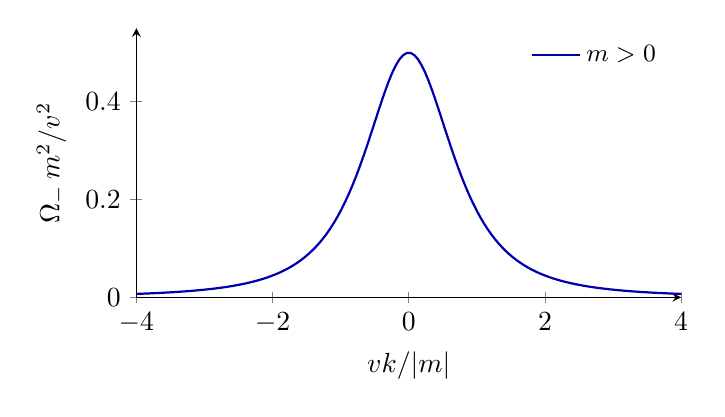
\begin{tikzpicture}
\begin{axis}[width=8.5cm,height=5cm,xlabel={$vk/|m|$},ylabel={$\Omega_-\,m^2/v^2$},axis lines=left,xmin=-4,xmax=4,ymin=0,ymax=0.55,domain=-4:4,samples=150,legend style={draw=none,font=\small}]
  \addplot[thick,blue!70!black] {0.5/(x^2+1)^1.5};
  \addlegendentry{$m>0$}
\end{axis}
\end{tikzpicture}
\caption{Berry curvature of the lower band of the massive Dirac Hamiltonian, for $m>0$. It is concentrated within $k\lesssim|m|/v$ of the band edge and integrates to $\pi$. For $m<0$ the curve is reflected through zero.}
\label{fig:dirac-curvature}
\end{figure}

\paragraph{Energy as the integration variable.} From $\varepsilon\,d\varepsilon = v^2k\,dk$,
\[
    \int\Omega_\pm\,k\,dk = \mp\frac m2\int\frac{d\varepsilon}{\varepsilon^2},
\]
with limits taken from $|m|$ (the band edge), $|E_F|$ (a Fermi circle) and $\infty$. The total over the plane for the lower band is:

\begin{theorem}[Half-quantized Berry flux]
\[
    \int_{\mathbb{R}^2}\Omega_-\,d^2k = 2\pi\cdot\frac m2\int_{|m|}^\infty\frac{d\varepsilon}{\varepsilon^2} = \pi\,\operatorname{sgn}m,
    \qquad
    \frac{1}{2\pi}\int\Omega_-\,d^2k = \tfrac12\operatorname{sgn}m .
\]
\end{theorem}

\paragraph{Why half.} As $k$ runs from $0$ to $\infty$, $\hat{\lvect{d}}$ runs from a pole to the equator, covering one hemisphere, so the flux is half of the $2\pi$ a full sphere would give. The plane is not a closed surface, so there is no contradiction with the integer Chern theorem.

\paragraph{How lattices reach integers.} Flipping the sign of $m$ changes the total by a full $2\pi$. In a lattice model the Brillouin zone is closed, and the Dirac points come in groups (for example two valleys); the Chern number is the sum of their half-integers, $\sum\frac12\operatorname{sgn}m_i$, plus any smooth background. Two valleys with the same mass sign give $C = \pm1$; with opposite signs, $C = 0$. Tuning one mass through zero closes the gap and changes $C$ by one: Chern numbers can change only where the gap closes.

\paragraph{Finite cutoff.} If the Dirac form is valid only below a cutoff $k_{\max}$, the total is $\pi\bigl(\operatorname{sgn}m - m/\sqrt{m^2+v^2k_{\max}^2}\bigr)$, already close to $\pi\operatorname{sgn}m$ once $k_{\max}\gg|m|/v$.

% ============================================================
\section{Anomalous Hall Conductivity of the Massive Dirac Model}
\label{sec:anomalous-hall}
% ============================================================

\subsection{Formula and Occupations}

The Berry curvature acts as a magnetic field in $\lvect{k}$-space. It adds an \emph{anomalous velocity} to the semiclassical equations of Chapter~\ref{ch:semiclassical}, $\dot{\lvect{r}} = \frac1\hbar\nabla_{\lvect{k}}\varepsilon_n - \dot{\lvect{k}}\times\bm{\Omega}_n$, transverse to the applied force. Summing it over occupied states in an electric field gives a Hall current even with no magnetic field:

\begin{formula}[Hall conductivity from Berry curvature]
\[
    \sigma_{xy} = \frac{e^2}{\hbar}\sum_{\pm}\int\frac{d^2k}{(2\pi)^2}\,f_\pm(\lvect{k})\,\Omega_\pm(\lvect{k})
    = \frac{e^2}{h}\sum_\pm\int_0^\infty k\,dk\,f_\pm(k)\,\Omega_\pm(k),
    \qquad
    f_\pm = \Theta\bigl(E_F - E_\pm(\lvect{k})\bigr).
\]
For filled bands over a closed Brillouin zone this is $\frac{e^2}{h}\sum_{n\,\text{occ}}C_n$, the TKNN formula.
\end{formula}

The occupation is $\Theta(E_F-E)$: occupied states lie \emph{below} the Fermi level. The two bands have different occupied regions, so each gets its own limits.

\begin{figure}[ht]
\centering
\begin{tikzpicture}[>=Stealth]
  \draw[->] (-3,0) -- (3,0) node[below] {$k$};
  \draw[->] (0,-2.6) -- (0,2.7) node[above] {$E$};
  \draw[thick,blue!70!black,domain=-2.6:2.6,samples=80] plot (\x,{sqrt(0.6*\x*\x+0.36)});
  \draw[thick,blue!70!black,domain=-2.6:2.6,samples=80] plot (\x,{-sqrt(0.6*\x*\x+0.36)});
  \draw[dashed,orange!70!black] (-3,1.3) -- (3,1.3) node[right] {$E_F>|m|$};
  \draw[dashed,orange!70!black] (-3,0.3) -- (3,0.3) node[right] {in gap};
  \draw[dashed,orange!70!black] (-3,-1.6) -- (3,-1.6) node[right] {$E_F<-|m|$};
  \node[left] at (-0.05,0.75) {\small $|m|$};
  \node[left] at (-0.05,-0.75) {\small $-|m|$};
\end{tikzpicture}
\caption{The massive Dirac bands $E_\pm = \pm\sqrt{v^2k^2+m^2}$ and the three positions of the Fermi level.}
\label{fig:dirac-bands}
\end{figure}

\subsection{The Three Regimes}

In units of $e^2/h$, using $\int\Omega_\pm k\,dk = \mp\frac m2\int\varepsilon^{-2}d\varepsilon$:
\begin{itemize}
    \item \textbf{$E_F$ in the gap:} lower band full ($k$ from $0$ to $\infty$), upper band empty:
    $\frac m2\int_{|m|}^\infty\varepsilon^{-2}\,d\varepsilon = \frac12\operatorname{sgn}m$.
    \item \textbf{$E_F>|m|$:} lower band full, upper band filled for $k<k_F$ with $vk_F = \sqrt{E_F^2-m^2}$:
    $\frac12\operatorname{sgn}m - \frac m2\bigl(\frac1{|m|} - \frac1{E_F}\bigr) = \frac{m}{2E_F}$.
    \item \textbf{$E_F<-|m|$:} only lower-band states with $\varepsilon>|E_F|$ are occupied:
    $\frac m2\int_{|E_F|}^\infty\varepsilon^{-2}\,d\varepsilon = \frac{m}{2|E_F|}$.
\end{itemize}

\begin{formula}[Anomalous Hall conductivity of a massive Dirac fermion]
\[
    \sigma_{xy} = \frac{e^2}{2h}\times
    \begin{cases}
        m/|E_F|, & E_F<-|m|,\\
        \operatorname{sgn}m, & |E_F|<|m|,\\
        m/|E_F|, & E_F>|m|,
    \end{cases}
    \qquad\text{i.e.}\qquad
    \sigma_{xy} = \frac{e^2}{2h}\,\frac{m}{\max(|m|,|E_F|)} .
\]
\end{formula}

\begin{figure}[ht]
\centering
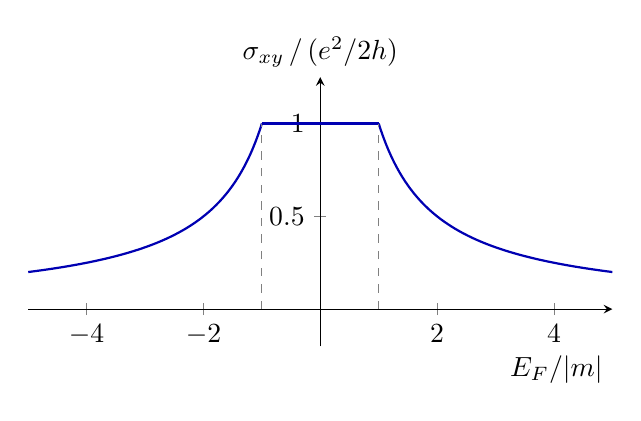
\begin{tikzpicture}
\begin{axis}[width=9cm,height=5cm,xlabel={$E_F/|m|$},ylabel={$\sigma_{xy}\,/\,(e^2/2h)$},axis lines=middle,xmin=-5,xmax=5,ymin=-0.2,ymax=1.25,samples=200,xlabel style={at={(1,0)},anchor=north east},ylabel style={at={(0.5,1)},anchor=south}]
  \addplot[thick,blue!70!black,domain=-5:-1] {1/abs(x)};
  \addplot[thick,blue!70!black,domain=-1:1] {1};
  \addplot[thick,blue!70!black,domain=1:5] {1/abs(x)};
  \addplot[dashed,gray] coordinates {(-1,0) (-1,1)};
  \addplot[dashed,gray] coordinates {(1,0) (1,1)};
\end{axis}
\end{tikzpicture}
\caption{Anomalous Hall conductivity of a massive Dirac fermion with $m>0$ as the Fermi level is moved. It is half-quantized in the gap and falls off as $1/|E_F|$ in either band.}
\label{fig:sigma-xy-dirac}
\end{figure}

Checks:
\begin{itemize}
    \item It is continuous at $|E_F| = |m|$.
    \item It is maximal, and half-quantized, in the gap.
    \item It decays as $1/|E_F|$ because the occupied curvature of the partly filled band cancels part of the full band's.
    \item It is symmetric between electron and hole doping.
    \item It is odd in $m$: the mass breaks time-reversal symmetry, without which $\sigma_{xy}$ must vanish.
    \item Its overall sign flips with the curvature convention.
\end{itemize}
The Fermi level can be on either side of zero: $E = 0$ is mid-gap, and $E_F$ is set by doping or gating. A single Dirac fermion can give only half a quantum; a gapped lattice model, with its closed Brillouin zone, gives an integer (previous section), and that integer is the plateau value of the quantum Hall effect.

% ============================================================
\section{Checklist of Pitfalls}
% ============================================================

\begin{enumerate}
    \item A Berry connection must be real. An imaginary result means a dropped factor of $i$.
    \item The $\phi\to\phi+2\pi$ wrap is harmless; the singularities of a gauge sit at points where $\phi$ is undefined (poles, $\lvect{k} = 0$).
    \item Gauge changes must be single-valued: $\delta$ may wind only by multiples of $2\pi$.
    \item Distinguish coordinate components (coefficients of $d\theta$, $d\phi$) from physical ones: divide by $\sin\theta$ on the sphere, and include the $1/k$ in the plane polar curl.
    \item Open-path Berry phases are gauge dependent; closed-loop phases are invariant modulo $2\pi$; curvature and its integrals are exactly invariant. State topological contradictions with curvature integrals.
    \item Keep track of whether the band is aligned ($-\frac12$ per solid angle) or anti-aligned ($+\frac12$) with $\hat{\lvect{d}}$; the sign of $H = \pm\lvect{d}\cdot\bm{\sigma}$ decides.
    \item Occupation is $\Theta(E_F-E)$, and each band gets its own limits.
    \item Keep $\sqrt{m^2} = |m|$; that is where the dependence on $\operatorname{sgn}m$ comes from.
\end{enumerate}

\begin{fact}[Key results of this chapter]
\begin{align*}
    &\bm{\mathcal{A}}_n = i\langle n|\nabla_{\lvect{R}}n\rangle,\quad \gamma_n = \oint\bm{\mathcal{A}}_n\cdot d\lvect{R}\ (\text{mod }2\pi) && \text{Berry connection and phase}\\
    &\bm{\Omega}_n = i\sum_{m\neq n}\frac{\langle n|\nabla H|m\rangle\times\langle m|\nabla H|n\rangle}{(E_n-E_m)^2},\quad \textstyle\sum_n\bm{\Omega}_n = 0 && \text{Berry curvature}\\
    &\gamma = \mp\tfrac12\,\Omega(C) && \text{spin-}\tfrac12\text{ (aligned/anti-aligned)}\\
    &\oint_S\bm{\Omega}_n\cdot d\lvect{a} = 2\pi C_n,\quad C_n\in\mathbb{Z} && \text{Chern number}\\
    &\Omega_\pm = \mp\frac{mv^2}{2(v^2k^2+m^2)^{3/2}},\quad \int\Omega_-\,d^2k = \pi\operatorname{sgn}m && \text{massive Dirac}\\
    &\sigma_{xy} = \frac{e^2}{2h}\frac{m}{\max(|m|,|E_F|)};\quad \sigma_{xy} = \frac{e^2}{h}\sum_{\text{occ}}C_n\ (\text{insulator}) && \text{anomalous Hall}
\end{align*}
\end{fact}
